\chapter{Bagging}\label{Chapter10} 
% chktex-file 8
% chktex-file 12
% chktex-file 13
% chktex-file 44

\section{Introducción}

El \textit{bootstrap} es una herramienta estadística muy poderosa de de gran aplicabilidad que sirve para cuantificar la incertidumbre asociada a un estimador o modelo de aprendizaje estadístico dado. Se utiliza en muchas situaciones en las que es difícil o incluso imposible calcular directamente la desviación estándar de una cantidad de interés. Vemos aquí que el bootstrap puede usarse con el fin de mejorar métodos de aprendizaje estadístico como los árboles de decisión. \\

Los árboles de decisión discutidos en el el capítulo \ref{Chapter6} sufren de alta varianza (si los hacemos crecer mucho, tenemos un modelo de alta varianza y bajo sesgo). Esto significa que si dividimos los datos de entrenamiento en dos partes al azar y ajustamos un árbol de decisión a ambas mitades, los resultados que obtenemos podrían ser bastante diferentes. En contraste, un procedimiento con baja varianza ofrecerá resultados similares si se aplica repetidamente a conjuntos de datos distintos; la regresión lineal tiende a tener baja varianza (si la proporción de $n$ a $p$ es moderadamente grande). La agregación, \textit{bootstrap}, o \textit{bagging}, es un procedimiento de propósito general para reducir la varianza de un método de aprendizaje estadístico particularmente útil y frecuentemente en el contexto de los árboles de decisión. \\

Dado un conjunto de $n$ observaciones independientes $Z_1, \ldots, Z_n$, cada una con varianza $\sigma^2$, la varianza de la media $\overline{Z}$ de las observaciones está dada por 
\begin{equation}
\sigma^2/n
\end{equation}

Es decir, promediar un conjunto de observaciones reduce la varianza. Por lo tanto, una forma natural de reducir la varianza y, por tanto, aumentar la precisión de predicción de un método de aprendizaje estadístico, es tomar muchos conjuntos de entrenamiento de la población, construir un modelo de predicción separado utilizando cada conjunto de entrenamiento, y promediar las predicciones resultantes. En otras palabras, podríamos calcular $\hat{f}_1(x)$, $\hat{f}_2(x)$, \ldots, $\hat{f}_B(x)$ usando $B$ conjuntos de entrenamiento separados, y promediarlos para obtener un único modelo de aprendizaje estadístico de baja varianza, dado por
\begin{equation}
\hat{f}_{\text{avg}}(x) = \frac{1}{B} \sum_{b=1}^{B} \hat{f}_b(x).
\end{equation}

Por supuesto, esto no es práctico porque generalmente no tenemos acceso a múltiples conjuntos de entrenamiento. En su lugar, podemos usar el \textit{bootstrap}, tomando muestras repetidas del conjunto de datos de entrenamiento (único), es decir, muestrear con remplazamiento: algunos ejemplos pueden no estar presentes en el conjunto de entrenamiento, y otros pueden estar duplicados, triplicados, etc. En este enfoque, generamos $B$ conjuntos de datos de entrenamiento \textit{bootstrap} diferentes (un \textit{bootstrap} para cada árbol del bosque). Luego entrenamos nuestro método en el conjunto de entrenamiento \textit{bootstrap} $b$ para obtener $\hat{f}^*_b(x)$, y finalmente promediamos todas las predicciones, para obtener
\begin{equation}
\hat{f}_{\text{bag}}(x) = \frac{1}{B} \sum_{b=1}^{B} \hat{f}^*_b(x).
\end{equation}

\noindent Esto se llama \textit{bagging}. \\

Mientras que el \textit{bagging} puede mejorar las predicciones para muchos métodos de regresión, es particularmente útil para los árboles de decisión, ya que tienen un \textit{bias} relativamente bajo si los dejamos crecer lo suficiente. Para aplicar \textit{bagging} a árboles de regresión, simplemente construimos $B$ árboles de regresión usando $B$ conjuntos de entrenamiento \textit{bootstrap}, y promediamos las predicciones resultantes. Estos árboles se crecen profundamente y no se podan. Por lo tanto, cada árbol individual tiene alta varianza, pero bajo sesgo. Promediar estos $B$ árboles reduce la varianza. El \textit{bagging} ofrece grandes mejoras en la precisión al combinar cientos o incluso miles de árboles en un solo procedimiento. \\

Hasta ahora, hemos descrito el procedimiento de bagging en el contexto de regresión, para predecir un resultado cuantitativo $Y$. Para extender el \textit{bagging} a un problema de clasificación donde $Y$ es cualitativo, el enfoque más sencillo es el siguiente. Para una observación de prueba dada, podemos registrar la clase predicha por cada uno de los $B$ árboles, y tomar una mayoría de votos: la predicción general es la clase que ocurre con mayor frecuencia entre las $B$ predicciones. Las predicciones que daremos serán: 
\begin{itemize}
\item Regresión: 
\begin{equation}
\hat{f}_{\text{bag}}(x) = \frac{1}{B} \sum_{b=1}^{B} \hat{f}^*_b(x)
\end{equation}
\item Clasificación. Sea $\hat{f}_{\text{bag}} (x)$ la proporción de árboles que predice cada clase, se toma la probabilidad media para cada clase:
\begin{equation}
\hat{G}_{\text{bag}}(x) = \text{argmax}_k \hat{f}_{\text{bag}} (x)
\end{equation}
\end{itemize}

\begin{figure}[h]
\centering
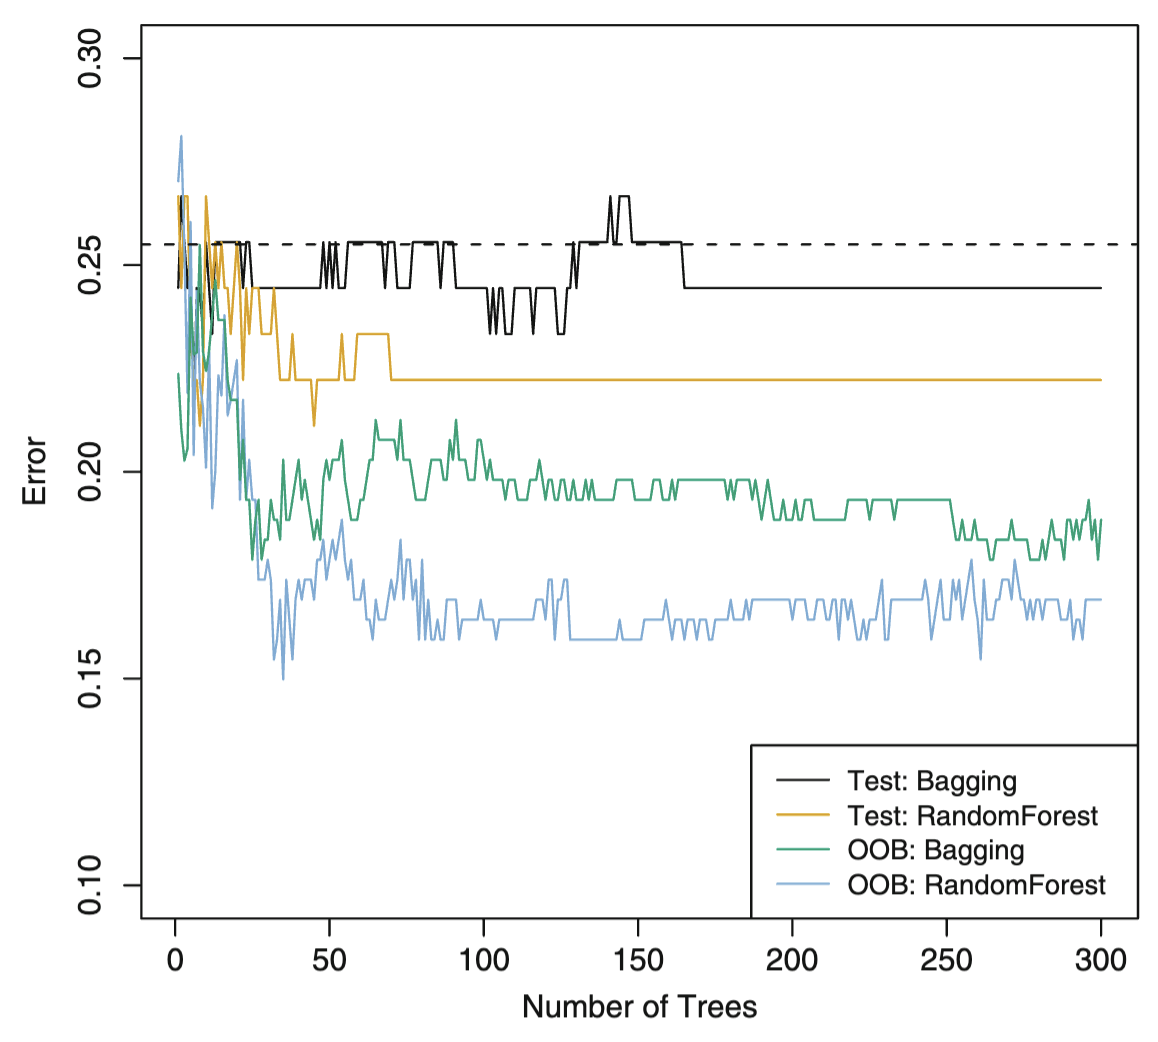
\includegraphics[width=0.5\textwidth]{fotos/59.png}
\caption{\textit{Bagging} y \textit{Random Forests} sobre los datos de \texttt{Heart}. El error de prueba (negro y naranja) se muestra como función de $B$, el número de conjunto de entrenamiento de \textit{bootstrap} usados. Se aplicaron \textit{Random Forest} con $m = \sqrt{p}$. La línea discontinua indica el error de prueba resultante de un único árbol de clasificación. Las líneas azul y verde muestran el error OOB, que resulta considerablemente menor en este caso. }
\label{fig:20.8}
\end{figure}

La figura 8.8 muestra los resultados del bagging de árboles en los datos de Heart. El número de árboles $B$ no es un parámetro crítico con el bagging; usar un valor muy grande de $B$ no llevará al sobreajuste. En la práctica, usamos un valor de $B$ suficientemente grande para que el error se haya estabilizado. Usar $B = 100$ es suficiente para lograr un buen rendimiento en este ejemplo.

\section{Random Forest}

Como ya comentamos, el \textit{bagging} parece funcionar especialmente bien para procedimientos de alta varianza y bajo sesgo, como los árboles. Para la regresión, simplemente ajustamos el mismo árbol de regresión muchas veces a versiones de los datos de entrenamiento muestreados por \textit{bootstrap}, y promediamos el resultado. Para la clasificación, un comité de árboles emite un voto para la clase predicha. \\

El \textit{boosting} se propuso inicialmente como un método de comité, aunque a diferencia del \textit{bagging}, el comité de aprendices débiles evoluciona con el tiempo, y los miembros emiten un voto ponderado. El \textit{boosting} parece dominar al bagging en la mayoría de los problemas, y se convirtió en la opción preferida. Los \textit{random forests} son una modificación sustancial del \textit{bagging} que construye una gran colección de árboles desacoplados y luego los promedia. En muchos problemas, el desempeño de los \textit{random forests} es muy similar al del \textit{boosting}, y son más sencillos de entrenar y ajustar. Como consecuencia, los \textit{random forests} son populares. 

\subsection{Definición}

La idea esencial en el \textit{bagging} es por tanto promediar muchos modelos ruidosos pero con bajo sesgo, y así reducir la varianza. Los árboles son candidatos ideales para el \textit{bagging}, ya que pueden capturar estructuras de interacción complejas en los datos y, si se crecen lo suficientemente profundos, tienen un sesgo relativamente bajo. Dado que los árboles son ruidosos, se benefician enormemente del promediado. Además, dado que cada árbol generado en el \textit{bagging} está identicamente distribuido (i.d., es decir, las muetstras de datos vienen de la misma distribución de probabilidad), la expectativa de un promedio de $B$ árboles es la misma que la expectativa de cualquiera de ellos. Esto significa que el sesgo de los árboles ``baggeados'' es el mismo que el de los árboles individuales, y la única esperanza de mejora es a través de la reducción de la varianza. Esto contrasta con el \textit{boosting}, donde los árboles se crecen de manera adaptativa para eliminar el sesgo, y por lo tanto no son i.d. \\

\noindent El \textit{random forest} introduce una aleatoriedad en el entrenamiento de cada árbol, para mantener baja la correlación y evitar el aumento de varianza. Tanto para clasificación como para regresión, sigue el siguiente proceso:
\begin{itemize}
\item Desde $b = 1$ hasta $B$:
\begin{itemize}
\item Dibuja una muestra de \textit{bootstrap} $Z^*$ de tamaño $N$ a partir de los datos de entrenamiento.
\item Crece un árbol de \textit{random forest} $T_b$ con los datos de \textit{bootstrap} siguiendo de forma iterativa los siguiente pasos para cada nodo terminal del árbol, hasta alcanzar el tamaño mínimo de nodo $n_{\text{min}}$:
\begin{itemize}
\item Selecciona $m$ variables al azar de las $p$ variables.
\item Escoge la mejor variable/punto de división entre las $m$.
\item Divide el nodo en dos nodos hijo.
\end{itemize}
\end{itemize}
\item Da como salida el conjunto (\textit{ensemble}) de árboles $\{T_b\}_{b=1}^B$.
\end{itemize}

\noindent Para hacer una predicción sobre un nuevo punto $r$: 
\begin{itemize}
\item Regresión:
\begin{equation}
\hat{f}_{\text{rf}}^B(x) = \frac{1}{B} \sum_{b=1}^{B} T_b(x)
\end{equation}
\item Clasificación: Sea $\hat{C}_b (x)$ la clase predicha por el árbol b-ésimo de \textit{random forest}. Entonces
\begin{equation}
\hat{C}_{\text{rf}}^B(x) = \text{voto mayoritario} \left\{ \hat{C}_b(x) \right\}_{b = 1}^B
\end{equation}
\end{itemize}

Para clasificación, promediamos el vector de probabilidad de cada árbol tenemos una estimación más fiable que con un voto mayoritario simple, ya que no es lo mismo que una clase gane con 0.5 que con 0.9. 
\begin{example}
Tomamos la decision con este vector promediado, no con la votacion mayoritaria.
\begin{table}[H]
\centering
\begin{tabular}{cccc}
\toprule
 & \textbf{Clase 1} & \textbf{Clase 2} & \textbf{Clase 3} \\
\midrule
\textbf{Árbol 1} & 0.5 & 0.3 & 0.2 \\
\textbf{Árbol 2} & 0.3 & 0.3 & 0.4 \\
\textbf{Árbol 3} & 0.4 & 0.1 & 0.5 \\
\midrule
\textbf{Promedio} & 0.4 & 0.23 & 0.37 \\
\bottomrule
\end{tabular}
\end{table} 
\end{example}

Una ventaja frente a \textit{boosting} es que aqui podemos paralelizar completamente el aprendizaje, ya que cada árbol se entrena de forma independiente, no como en \textit{boosting} que se entrena de forma secuencial. Otra ventaja: no hay que usar un conjunto de validación para conocer el error: el error de \textit{out-of-bag} es una estimación no sesgada del error de prueba. \\

Por tanto, al usarse para clasificación, el \textit{random forest} obtiene un voto de cada árbol y clasifica usando la clase más votada. Al usarse para regresión, la predicción de cada árbol se promedia. Además, generalmente se suelen usar los siguiente valores para el número de variables a escoger $m$ y el tamaño mínimo de nodo $n_{\text{min}}$:
\begin{itemize}
\item Clasificación: $m = \lfloor\sqrt{p}\rfloor$ y $n_{\text{min}} = 1$.
\item Regresión: $m = \lfloor p/3\rfloor$ y $n_{\text{min}} = 5$.
\end{itemize}

Un promedio de $B$ variables aleatorias i.i.d., cada una con varianza $\sigma^2$, tiene una varianza de $\frac{1}{B} \sigma^2$. Si las variables son simplemente i.d. (idénticamente distribuidas, pero no necesariamente independientes) con correlación positiva por pares $\rho$, la varianza del promedio es
\begin{equation}
\frac{\rho \sigma^2 + (1 - \rho)}{B} \sigma^2
\label{eq:15.1}
\end{equation}

\begin{itemize}
\item Para árboles i.i.d., la correlación $\rho = 0$ y la varianza se reduce a $\sigma^2/B$. Esto ocurre al principio cuando hay pocos árboles.
\item Para árboles altamente correlacionados, $\rho \approx 1$, y la varianza del modelo total tiende a $\sigma^2$, lo que significa que no hay reducción de varianza.
\end{itemize}

A medida que $B$ aumenta, el segundo término desaparece, pero el primero permanece y, por lo tanto, el tamaño de la correlación de pares de árboles ``baggeados'' limita los beneficios del promediado (es decir, se reduce la varianza, pero hasta un límite). La idea en los \textit{random forests} es mejorar la reducción de varianza del \textit{bagging} al reducir la correlación entre los árboles, sin aumentar demasiado la varianza. Esto se logra en el proceso de crecimiento de los árboles mediante la selección aleatoria de las variables de entrada. Específicamente, al crecer un árbol en un conjunto de datos bootstrap, antes de cada división, seleccionamos $m \leq p$ de las variables de entrada al azar como candidatas para la división. Generalmente, los valores para $m$ son $\sqrt{p}$ o incluso tan bajos como 1.\\

Después de que crecer $B$ árboles $\{T(x; \Theta_b)\}_{b=1}^B$, el predictor del \textit{random forest} (regresión) es
\begin{equation}
\hat{f}_{\text{rf}}(x) = \frac{1}{B} \sum_{b=1}^{B} T(x; \Theta_b)
\label{eq:15.2}
\end{equation}

$\Theta_b$ caracteriza el $b$-ésimo árbol del \textit{random forest} en términos de variables de división, puntos de corte en cada nodo, y valores de los nodos terminales. Intuitivamente, reducir $m$ reducirá la correlación entre cualquier par de árboles en el conjunto, y por lo tanto, según (\ref{eq:15.1}), reducirá la varianza del promedio. \\

\begin{figure}[h]
\centering
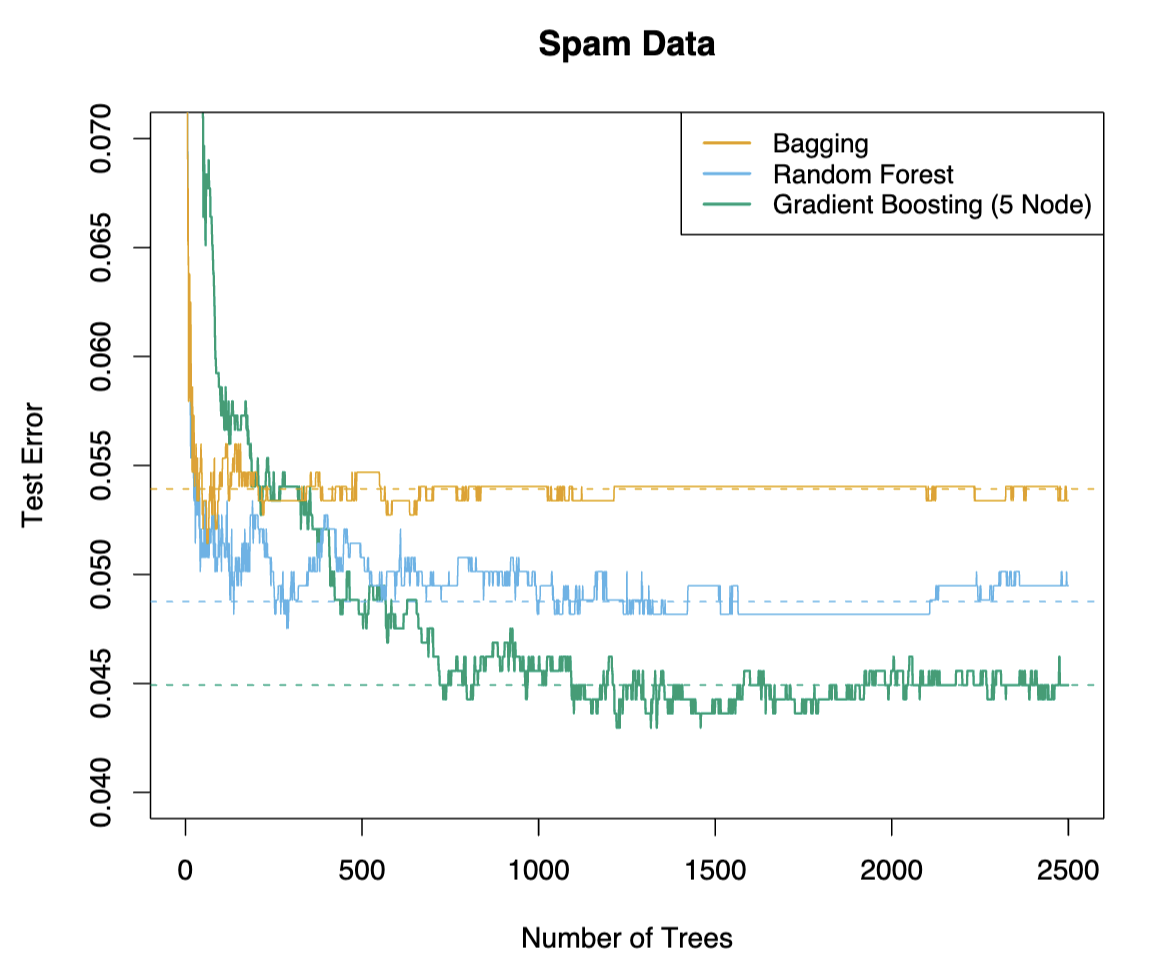
\includegraphics[width=0.5\textwidth]{fotos/60.png}
\caption{\textit{Bagging}, \textit{random forest} y \textit{gradient boosting} en el conjunto de datos de \texttt{Spam}. Para \textit{boosting} se usaron árboles de 5 nodos, y el número de árboles se escogió por validación cruzada con 10 pliegues (2500 árboles). Cada paso en la figura corresponde a el cambio en una única mala clasificación (en un conjunto de prueba de 1536 observaciones).}
\label{fig:20.9}
\end{figure}

No todos los estimadores pueden mejorarse agitando los datos de esta manera. Parece que los estimadores altamente no lineales, como los árboles, se benefician más. Para los árboles \textit{bootstrap}, $\rho$ es típicamente pequeño (generalmente 0.05 o menor; ver Figura 15.9), mientras que $\sigma^2$ no es mucho mayor que la varianza del árbol original. Por otro lado, el \textit{bagging} no cambia las estimaciones lineales, como la media muestral (y por lo tanto su varianza tampoco); la correlación por pares entre medias bootstrap es de aproximadamente 50\%. 

\subsection{Muestras \textit{out of bag}}

Una característica importante de los \textit{random forests} es el uso de muestras \textit{out-of-bag} (OOB): para cada observación $z_i = (x_i, y_i)$, se construye su predictor de \textit{random forest} promediando únicamente aquellos árboles correspondientes a muestras \textit{bootstrap} en las que $z_i$ no apareció (ya que de forma natural, \textit{bootstrap} excluye algunas observaciones). \\

Una estimación de error OOB es casi idéntica a la obtenida mediante validación cruzada de $N$ pliegues. Por lo tanto, a diferencia de muchos otros estimadores no lineales, los \textit{random forests} pueden ajustarse en una sola secuencia, realizando la validación cruzada en el camino. Una vez que el error OOB se estabiliza, el entrenamiento puede terminarse. La figura \ref{fig:20.4} muestra el error de clasificación OOB para los datos de spam, comparado con el error de prueba. Aunque aquí se promedian 2500 árboles, parece por el gráfico que alrededor de 200 serían suficientes.

\begin{figure}[h]
\centering
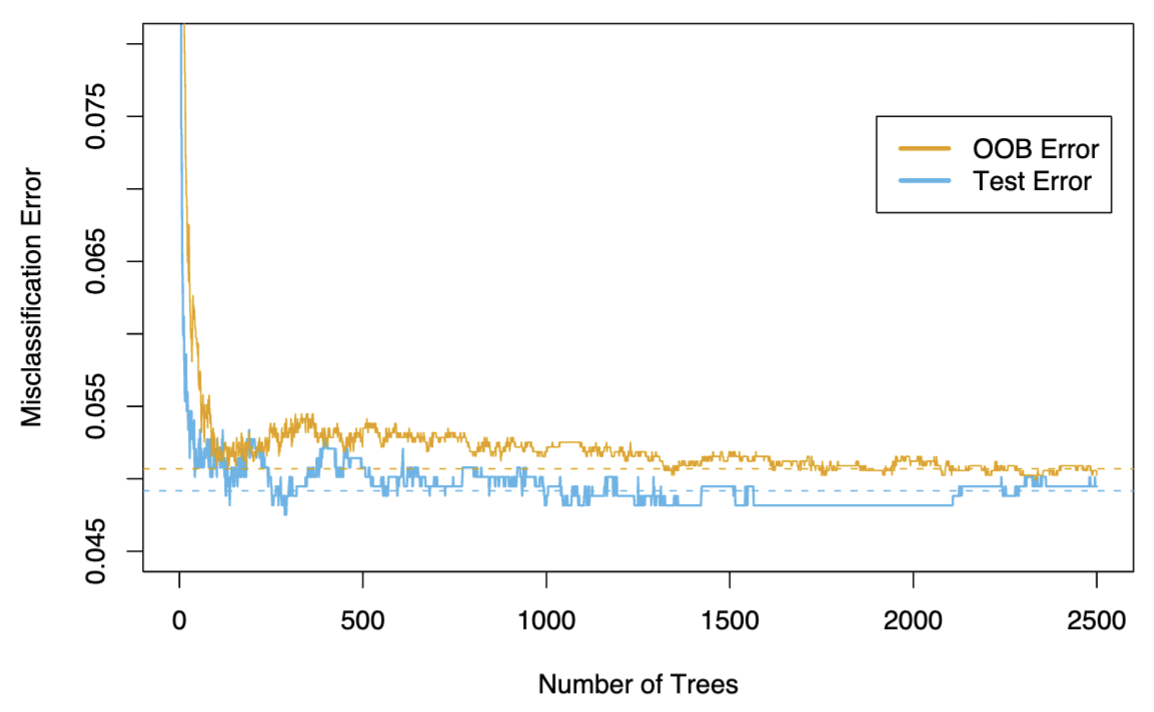
\includegraphics[width=0.5\textwidth]{fotos/61.png}
\caption{Error de clasificación OOB y error de prueba en el conjunto de datos de \texttt{Spam}.}
\label{fig:20.4}
\end{figure}


\subsection{Sobreajuste en \textit{random forest}}

Cuando el número de variables es grande, pero la fracción de variables relevantes es pequeña, es posible que los \textit{random forest} tengan un rendimiento deficiente con $m$ pequeño. En cada división, la probabilidad de que se seleccionen las variables relevantes (que den información para dar la respuesta) puede ser baja. La figura \ref{fig:20.7} muestra los resultados de una simulación que respalda esta afirmación. En la parte superior de cada par, vemos la probabilidad hipergeométrica de que una variable relevante sea seleccionada en cualquier división por un árbol de \textit{random forest} (en esta simulación, las variables relevantes son todas iguales en importancia). A medida que esta probabilidad disminuye, la brecha entre \textit{boosting} y los \textit{random forest} aumenta. Cuando el número de variables relevantes aumenta, el rendimiento de los \textit{random forest} es sorprendentemente robusto ante un incremento en el número de variables de ruido. Por ejemplo, con 6 variables relevantes y 100 de ruido, la probabilidad de que se seleccione una variable relevante en cualquier división es 0.46, asumiendo $m = \sqrt{6 + 100} \approx 10$. Según la figura \ref{fig:20.7}, esto no perjudica el rendimiento de los \textit{random forest} en comparación con el \textit{boosting}. Esta robustez se debe en gran medida a la relativa insensibilidad del costo de la mala clasificación al sesgo y la varianza de las estimaciones de probabilidad en cada árbol. Sin embargo, en un bosque esta insensibilidad se pierde, y el rendimiento de los \textit{random forest} se deteriora con el incremento del número de variables irrelevantes. \\

\begin{figure}[H]
\centering
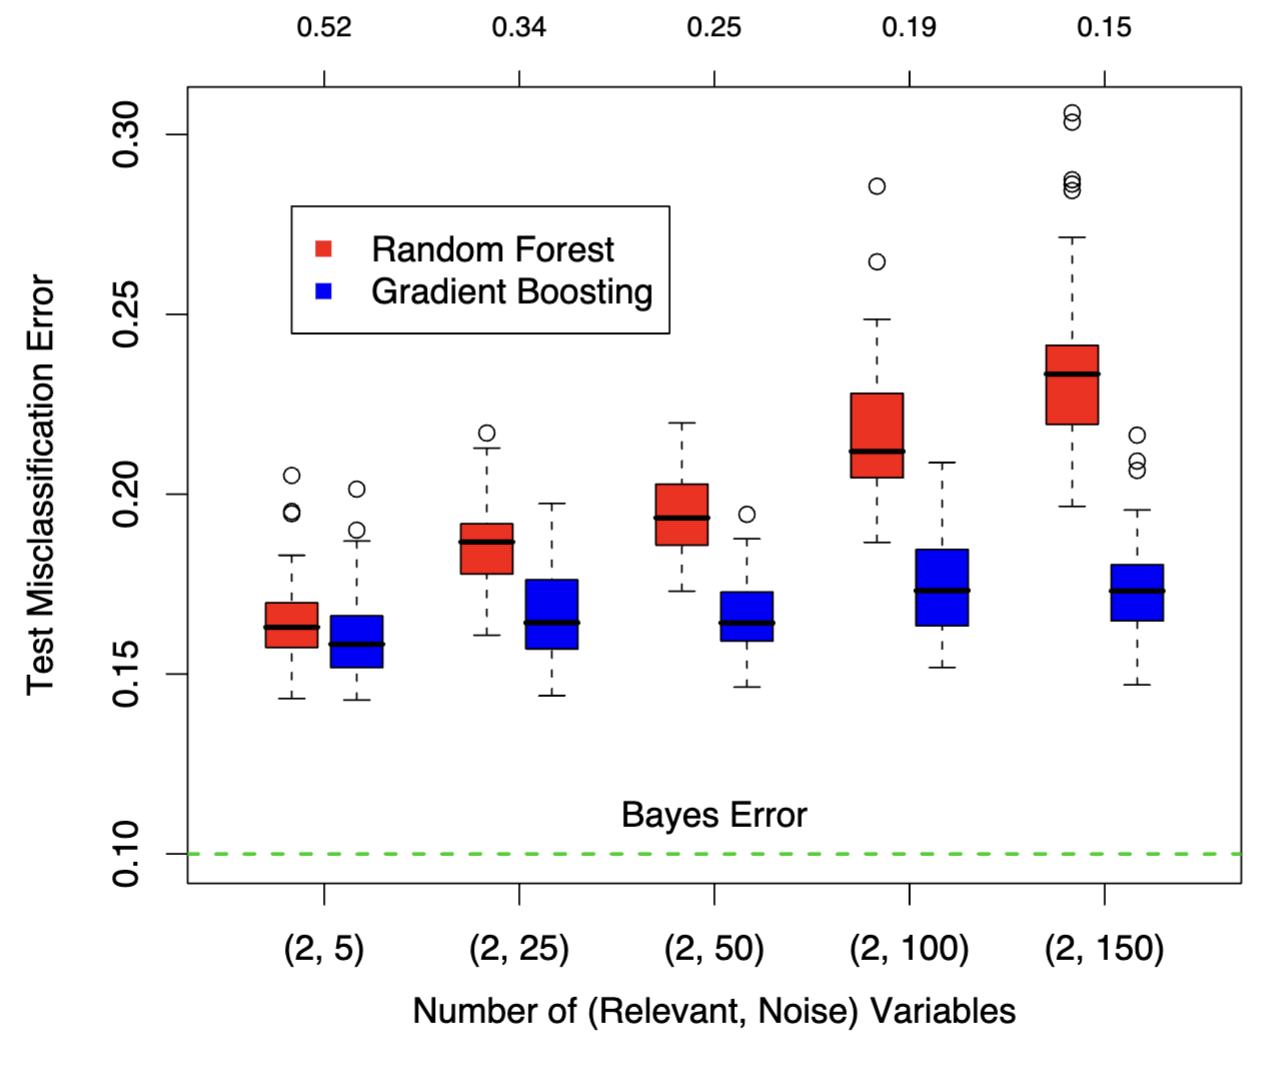
\includegraphics[width=0.5\textwidth]{fotos/62.png}
\caption{Comparación de \textit{random forest} y \textit{gradient boosting} en un problema con número creciente de variables con ruido. En cada caso, la frontera de decisión verdadera depende de dos variables, y se incluye un número creciente de variables con ruido. \textit{Random forest} usa el valor por defecto $m = \sqrt{p}$. Sobre cada par se muestra la probabilidad de elegir una variable relevante en una división o \textit{split}. Los resultados se basan en 50 simulaciones para cada par, con un conjunto de entrenamiento de 200 y un conjunto de prueba de 500.}
\label{fig:20.7}
\end{figure}

\begin{figure}[H]
\centering
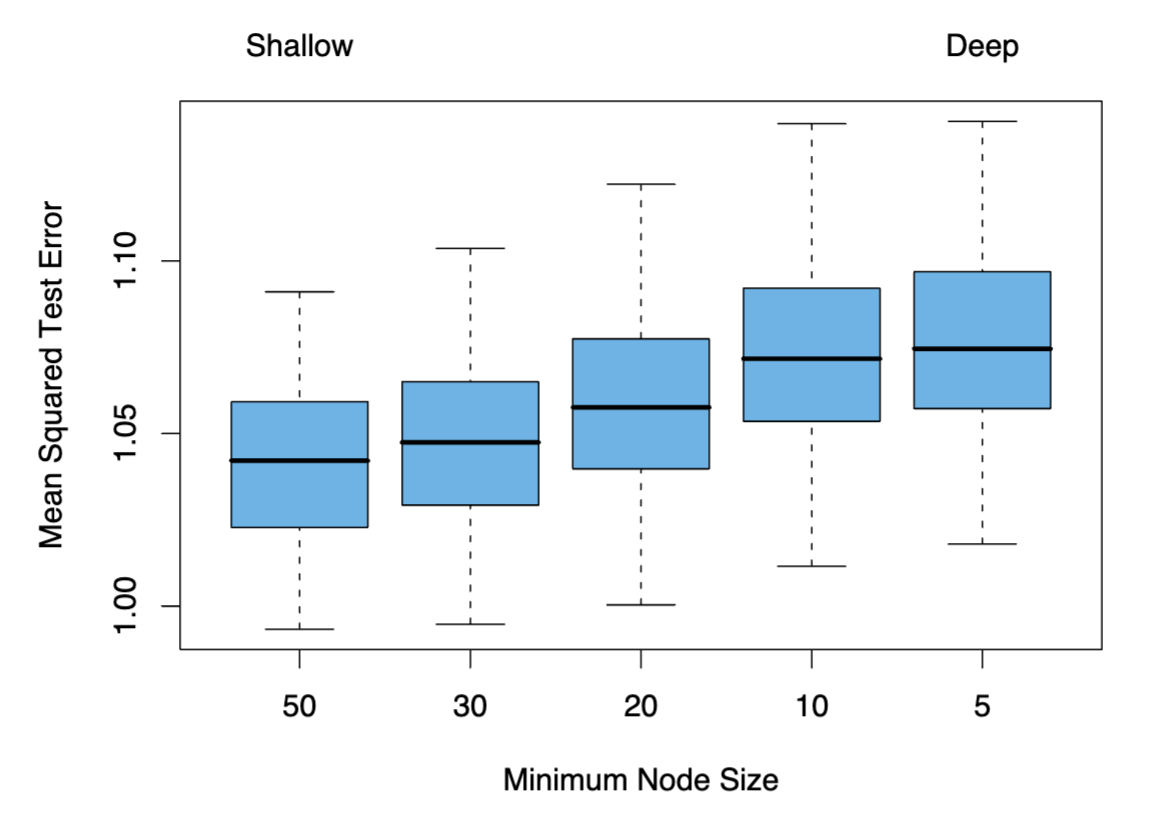
\includegraphics[width=0.5\textwidth]{fotos/63.png}
\caption{Efecto del tamaño del árbol sobre el error en regresión con \textit{random forest}. En este ejemplo, la superficie real era aditiva en 2 de las 12 variables, además de ruido gaussiano aditivo de varianza unitaria. La profundidad del árbol se controla aquí por el tamaño mínimo del nodo; cuanto menor sea el tamaño mínimo del nodo, más profundos serán los árboles.}
\label{fig:20.18}
\end{figure}

Una creencia común es que los \textit{random forest} ``no pueden sobreajustar'' los datos. Es cierto que aumentar $B$ no provoca que la secuencia de \textit{random forest} sobreajuste; al igual que el \textit{bagging}, la estimación de \textit{random forest} (\ref{eq:15.2}) aproxima la expectativa
\begin{equation}
\hat{f}_{rf} (x) = \mathbb{E}_{\Theta^T} (x; \Theta) = \lim_{B \to \infty} \hat{f} (x)_B^{rf}
\end{equation}

con un promedio sobre $B$ realizaciones de $\Theta$. La distribución de $\Theta$ aquí es condicional a los datos de entrenamiento. Sin embargo, este límite $B$ puede sobreajustar los datos si es muy grande; el promedio de árboles totalmente crecidos puede resultar en un modelo demasiado complejo, e
incurrir en una varianza innecesaria. \\

Existen pequeñas ganancias en rendimiento al controlar las profundidades de los árboles individuales cultivados en \textit{random forest}. Sin embargo, usar árboles totalmente crecidos rara vez cuesta mucho, y resulta en un parámetro de ajuste menos. Por tanto, en general, Lo normal es tratar con árboles relativamente grandes, no compensa el esfuerzo de controlar la profundidad.

La figura \ref{fig:20.18} muestra el efecto modesto del control de profundidad en un ejemplo simple de regresión. Los clasificadores son menos sensibles a la varianza, y este efecto de sobreajuste raramente se observa con la clasificación de \textit{random forest}. 




\section{18/12}

